\documentclass[a4paper, 11pt]{article}
\usepackage[pdftex]{graphicx}
\begin{document}
\section{Correctness}

{Correctness}: A sequence of transactions are said to be consistent if and only if a total ordeing of them according to precedence relationship can be established that demonstrates the same behavior as the execution of the program. Behavior for an operation means the data it has read or wants to write. Demonstrating the same behavior thus means all the read operations should still see the same data in the new sequence as they have seen in the actual sequence. However writs always writes the same value no matter what. Hence the behavior of a write operation is not alterable.\\

\textbf{Def 1-} \emph{Set of Primitive Operations}: Operations are taken from the set \{force-readoffset(filedescriptor), writeoffset(filedescriptor), readdata(inode, offset, length), writedata(inode, offset, length), commit\}.\\

\textbf{Def 2-} \emph{Set of User-Level Operations}: User-Level Operations are taken from the set \{Read(fildescriptor), GetFilePointer(filedescriptor), Write(filedescriptor), Seek(filedescriptor), EndTransaction\}.\\

\textbf{Note 1-} \emph{Assignment Operations Need Not Be Shown In $OP_{excecuted}$}: Operations like offset = offset + length and other assignment operations in $OP_{T_i}$ need not be shown in the actual sequence of operations namely $OP_{executed}$ that consists of operations executed by different transaction so far, the reason is simply all such operations are local to the transaction and do not affect any other transaction's state and hence do not restrict the commution of other operations in any manner.\\

\textbf{Note 2} \emph{Forced-Readoffset(fd)}: Reads the offset for the filedescriptor and makes the transaction bound to this value.\\

\section{FileDescriptor Offset State per Transaction}:

Each filedescriptor has an associated offset with it, within each transaction this offset can be in 4 different states, these states indicate the dependency the transaction has on the value of this offset:\\

1- \textbf{No Access}: This is the default state for all filedescriptors in a transaction and is changed as soon as there is an access to the the descriptor within the transaction (any of the use-level operations are invoked).\\

2- \textbf{None}: Meaning there is no dependency for any operation in this transaction on the value of the offset associated with this descriptor regarding other transactions.\\ %This stems from the fact that the offset has been assigned an absolute value in this transaction and no operation reads on the value the offset had before this transaction accessed it.\\

3- \textbf{Write Dependency}: This kind of dependency means there is at least one operation in $OP_{T_i}$ having an unknown offset(essentially a write operation) value as argument. The value of this unknown offset will be determined at commit instant. \\

4- \textbf{Read Dependency}: This kind of dependency means there is at least one operation acting on an offset value for fd, where the value for fd has been determined by a previously committed transaction.\\


The state machine below depicts the behavior of the user level operations regarding how the offset corresponding to that transaction changes: \\

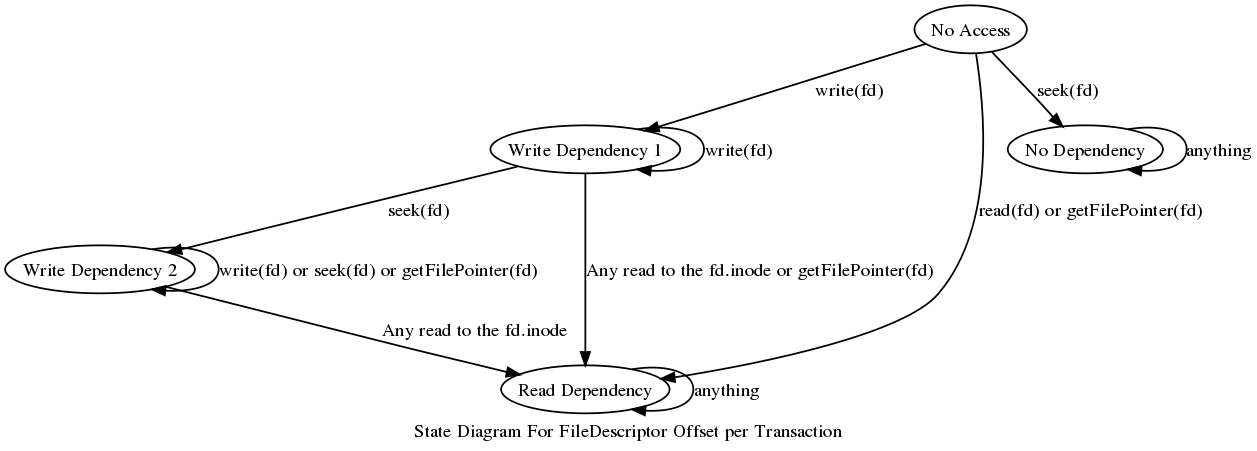
\includegraphics[scale = 0.3]{hello.png}\\

\textbf{Explanation}: Whenever the offset status for the transaction goes to "Read Dependence", a "forced-readoffset(fd)" operation is issued immediately preceding the operation that caused this transformation. The forced-radoofset(fd) is only issued if there is not a forced-readoffset(fd) in the $OP_{T_i}$ already.\\ 

\textbf{Axiom For Diagram:} If the first access to a filedescriptor is a $Seek(fd)$, then the following operation on $fd$ gets the offset value from the assignment made by the $Seek(fd)$ and advances the offset. Hence, the following operations get this offset and the offset value the filedescriptor had had before this transaction accesses fd is never referenced (thats why it is an absorbing state). This conforms to the definition of "None" state.\\ 

If $Read(fd.inode, offset, length)$ or $GetFilePointer(fd)$ is the first access made by this transaction, the offset is read (since the data needs to be read at this instant), this offset should be the one committed by a previously committed transaction (as this is the first access to $fd$ in this transaction). Once the offset is read, it is always dependent on this value (hence an absorbing state). For all the following operations, the offset value is known. This conforms to the definition that there is at least (the first read ever on fd by this transaction) one operation that acts on the offset value for fd and rules out the "Write Dependency" and "None" states.\\

If $Write(fd.inode, offset, length)$ is the first access made to fd by this transaction, then the offset to write to, can be decided at commit instant since the Write functions means start writing at the most recent committed fd.offset, hence offset realization can be postponed till commit instant. Any Writes or Seeks would still leave this dependency, since operations after a Seek act on absolute offset, and Writes preceding any Seek can all determine the offset at commit instant for the same reason as before.\\    

However, if a Read on the same fd in the transaction is invoked there are two possibilities:\\

1- A Seek precedes this Read, hence the offset value is absolute and is not read, however the ranges that are supposed to be written by Writes preceding the Seek, may overlap with the range Read is willing to Read from, and according to Rules(Most Recent Changes Should Be Visible) if thats the case the Read should be able to see this data, this suggests the ranges that all the Writes are going to write to should be realized now and this requires settling down on a value for all file descriptors offsets for this inode at this instant. Based on these, the most recent committed offset value for all these descriptors should be assigned to the offsets for the Writes that for the first time accessed the descriptor. Other for writes preceding the Seek, get this value as being advance by prior writes.\\

2- No Seek precedes the Read, hence the offset value the Read has to read from is unknown, since preceding Writes to fd have all used unknown offsets, the offset value given to Read is an unknown once, however it has to be known, follows that the offset value for the Write that for the first time accessed this fd should be decided upon and as shown before, the value should be the most recent committed offset value for fd. The offset value for this read or other writes, is the offset value obtained as being advanced by those operations.\\  

The two same possibilities exist when a GetFilePointer operation is invoked on the same fd:\\

1- If a Seek precedes it, then the offset value becomes absolute and hence the getFilePointer could retrieve the value assigned by Seek.\\

2- Otherwise, the offset value is still unknown, hence to be able to determine the offset value at this instant, the value obtained by reading the last committed offset value should be assigned to the offset value. for the first Write to $fd$.\\



%\textbf{Def 2-} \emph{Read and Write Operation}: 1- A Readdata is always a read operation. 2- ${readoffset(fd})\in OP_{T_i}$ is only a read operation, if it precedes a ${forceoffset(fd)} \in OP_{T_i}$. The reason is even though readoffset reads the offset, but the value does not matter unless specefied by ${forceoffset }$. 3- ${writeoffset}$ and ${writedata}$ are write operations.\\


%\textbf{Note 1-}: The runtime determines if and only if this is the first time the fd has been accessed by this transaction, then a $\{{offset} = {readoffset(fd)}\}$ is inserted in the sequence of operations. This ensures the offset is read for each filedescriptor once, and thats the first time it is accessed.\\

\section{User-Level Operations Structure}

The user-level operation cab be broken as follows:\\

1- Seek(fd): This operation sets the offset for filedescriptor. We define it as demonstarted below:\\

\hspace{8mm} Just an internal assignment in the transaction, $\{{fd.offset = value}\}$.\\  


2- Write(fd):\\

\hspace{8mm} 1- $\{writedata(fd.inode, offset, length), fd.offset = fd.offset + length\}$\\

3- GetFilePointer(fd):\\

\hspace{8mm} \{\{$forcedreadoffset(fd)$ issued as demonstrated at the state diagram if any, it is issued when the state for fd in this transaction is not in "No Dependency" or "Write Dependency 2"\}\}\\

4- Read(fd):\\

\hspace{8mm} $\forall filedescriptor fd_i$ where $fd_i.inode = fd.inode$ and the state for $fd_i$ in this transaction is not $No Dependency$, Read(fd) =$\{\{forcedreadoffset(fd_i)\}\}, {readdata(fd.inode, offset, length)}, offset = offset + length\}$\\

%\hspace{8mm}  1-  If ${read(fd)} \in OP_{T_i}$ and  $\exists forceoffset(fd) \in OP_{T_i}$ such that $forceoffset(fd) \rightarrow read(fd)$, then:\\

%\hspace{16mm} $\{{read(fd)}=readdata(fd.inode, offset, lenght), fd.offset = fd.offset + length\} $\\


%\hspace{8mm}  2-  If ${read(fd)} \in OP_{T_i}$ and  $ \not \exists forceoffset(fd) \in OP_{T_i}$ such that $forceoffset(fd) \rightarrow read(fd)$, then:\\

%\hspace{16mm} 1- If $\exists Seek(fd) \in USEROP_{T_i}$ such that $Seek(fd) \rightarrow read(fd)$ then:\\  

%\hspace{16mm} $\forall fd_i \in filedescriptors-accessed-by-T_i$ if $\exists writedata(fd_i.inode, offset, length)$ where $fd_i.inode = fd.inode$ and ${write(fd_i, offset, lenght)} \rightarrow {read(fd)}$  and $\not \exists seek(fd_i)$ such that $seek(fd_i) \rightarrow write(fd_i)$ and $\not \exists forceoffset(fd_i)$ such that $forceoffset(fd_i) \rightarrow read(fd)$ then ${read(fd)} = \{ \{forceoffset(fd_i)\},readdata(fd.inode, offset, length), fd.offset = fd.offset + length\}$ \\

%\hspace{16mm} 2- Else:\\ $\forall fd_i \in filedescriptors-accessed-by-T_i$ excluding $fd$ itself, if $ \exists writedata(fd_i.inode, offset, length)$ where ${write(fd_i, offset, lenght)} \rightarrow {read(fd)}$  and $\not \exists seek(fd_i)$ such that $seek(fd_i) \rightarrow write(fd_i)$ and $\not \exists forceoffset(fd_i)$ such that $forceoffset(fd_i) \rightarrow read(fd)$ then ${read(fd)} = \{ \{forceoffset(fd_i)\},readdata(fd.inode, offset, length), fd.offset = fd.offset + length\}$ \\

5- EndTransaction: 

\hspace{8mm} $\forall fd_i$ such that the state for $fd_i$ in this transaction is  not "No State",  $EndTransaction= \{\{{writeoffset(fd_i)}\}, commit\}$\\

Essentially for any fd that the correspondent state diagram in the transactions shows is in a state other than "No Access", a writeoffset(fd) is issued while committing.\\



\section{FileDescriptor Offset State per writedata Operation}

Any writedata operation within a transaction gets $fd$ and an offset as arguments. There writes are reflected in the commit instant, however the offset to write to as we saw earlier for some writes i s determined at commit instant and for other is bound to a specific value before commit instant. We should have a policy to be able to diffrenciate between these two. The 3 rules below odes this.\\

1- If the state for $fd$ a given distinguish in a transaction is "Write Dependency 1" all writes by that transaction to that $fd$ will get the value of the offset to write to at commit instant (since in "Write Dependency 1" all writes are at unknown offsets) .\\\

2- If the state for $fd$ is "Read Dependency"  or "No Dependency" then all writes on $fd$ within this transaction should be done at offset determined for them when they were invoked (since all writes are to known offsets either determined by the transaction itself or a previously committed transaction).\\

3- Otherwise, if the state is "Write Dependency 2", then if the $writedata(fd.inode,...)$ operation precedes a $Seek(fd)$ then the offset is determined at commit instant (since all such writes are at unknown offset). Otherwise, the writes should be done at the offset decided upon earlier (the write after a Seek write the offset determined by Seek and hence to a known offset).\\


We could also think of this as a state machine for each writedata operation. The state diagram is created for each operation when it is first invoked and is subject to two things:\\

1- If there $\exists Seek(fd) or forced-readoffset(fd)\in OP_{T_i}$ such that those precede the $writedata(fd.inode,....)$ then the initial state in the state diagram for this writedata is Absolute.\\

2- Otherwise the initial state is Unknown offset.\\

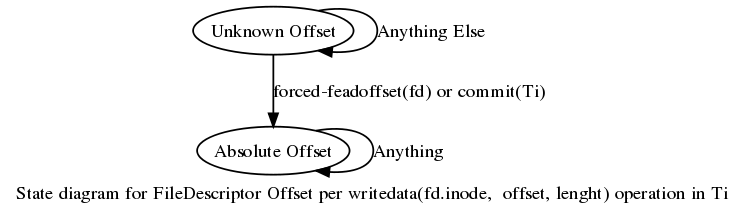
\includegraphics[scale = 0.3]{hello2.png}\\

\section{Commuting Operations}

As we saw earlier in Rule 4, any two operations can commute across each other unless they are subject to one of the two conditions in Rule 3.\\  

\textbf{Guideline 1}: \emph{Commuting forced-readoffset Operations}: A $forced-readoffset(fd) \in OP_{T_i}$ can go past a $commit_{T_j}$ if and only $\not \exists writeoffset(fd) in OP_{T_j}$.\\

\textbf{Axiom}: It follows immediately from Rule 4 and conditions in Rule 3, that this $forced-readoffset(fd)$ can go pats the commit. What remains to be proven is  $ \not \exists writeoffset(fd) \in OP_{T_i}$ such that it precedes 
$forced-readoffset(fd)$, as this would mean even if $\exists writeoffset \in OP_{T_j}$ still the $forced-readoffset(fd)$ could commute with $commit_{T_j}$.\\

This stems from the definition of EndTransaction operation, and the state diagram. A $forced-readoffset$ can be issued at any place in $OP_T{i}$ however it would always precede the $writeoffset(fd) \in OP_{T_i}$ since this is last operation in $OP_{T_i}$ before $commit$.\\

\textbf{guideline 2}: \emph{Commuting readdata Operations}:% A $readdata(fd_i.inode,offset_i, lenght_i) \in OP_{T_i}$ can go past a $commit_{T_j}$ if and only if $\not \exists writedata(fd_j.inode, offset_j, length_j) in OP{T_j}$ such that fd_j.inode= fd_i.inode and the two ranges (offset_i, offset_i + length_i) and (offset_i, offset_j + length_j) have an intersection.\\

%\textbf{Axiom}:\ This is 

\end{document}
